\chapter{Problemak.}

\section{Sarrera.}


%Josebaren zuzenketa 08-05-2017
%Tesiaren erdigunea N-gorputzeko problema grabitazionala da. Gure helburua, eguzki-sistemaren problemaren simulaziorako zenbakizko integratzaile eraginkorra inplementatzea da. Eguzki-sistemaren bi eredu sinple kontsideratu ditugu: lehena, \emph{kanpo-planeten} izeneko problema (eguzkia, kanpo-planetak eta Plutonek osatutakoa), eta bigarren eredu konplexuagoa, \emph{9-planeten problema} izeneko problema (eguzkia, 8 planetak eta Plutonek osatutakoa). Bi eredu hauetan, gorputzak masa puntualak dira eta gorputz hauen arteko erakarpen grabitazionalak bakarrik kontsideratu ditugu (erlatibitate efektua eta beste hainbat indar ez-grabitazionalak gure lan-eremutik kanpo utzi ditugu).

%Josebaren zuzenketa.
Gure helburua eguzki-sistemaren simulaziorako zenbakizko integratzaileak hobetzea eta hobekuntza horiek barneratzen dituen inplementazioa eskaintzea da. Eguzki-sistematzat nahi bezain konplexua den sistema har daiteke: planeta guztiak, planeta nanoak, planeten ilargiak, kometak, erlatibitate efektua eta abar har daitezke kontutan. Baina sistema sinplifikatuan hobekuntzak egiten badira, sistema konplexuak ere hobeto integratzeko bidea irekiko da. Hori dela-eta, guk eredu sinpleekin jardun dugu. Esate baterako, eguzki-sistemaren bi eredu sinple kontsideratu: kanpo-planeten problema (eguzkia, kanpo-planetak eta Plutonek osatutakoa), eta bigarren eredua, \emph{9-planeten problema}  problema (eguzkia, 8 planetak eta Plutonek osatutakoa).  Bi eredu hauetan, gorputzak masa puntualak dira eta gorputz hauen arteko erakarpen grabitazionalak bakarrik hartu ditugu kontutan.

Aipatu beharra dago, zenbakizko metodo sinplektiko nagusienak esplizituak direla eta metodo horiek, Hamiltondar banagarria duten problemetan bakarrik erabil daitezkeela. Gainera, problema zurruna bada metodo esplizituak ez dira eraginkorrak eta metodo inplizituek abantaila azaltzen dute. Gauss metodoa, orokorra  eta inplizitua izanik, problema zurrunetarako eta Hamiltondar banagarria ez den problemetarako  aplikagarria dela ere erakutsi nahi dugu. 
 
Hori dela-eta, problema osagarri gisa aukeratu dugu pendulu bikoitzaren problema, zenbakizko esperimentuak modu aberatsago eta zabalago batean egiteko. Pendulu bikoitzaren bi bertsio kontsideratu ditugu: pendulu bikoitz arrunta eta pendulu bikoitz zurruna.

N-gorputzeko problema grabitazionalaren Hamiltondarra banagarria da baina pendulu bikoitzarena aldiz, ez da banagarria. Bestalde, pendulu bikoitzari malguki bat gehituz  problema zurruna bilakatuko dugu, problema hauen zailtasunei nola aurre egin erakusteko. Gainera,  eguzki-sistema kaotiko \cite{Laskar1999}  kontsideratzen dela  jakinik, pendulu bikoitz arruntak izaera kaotikoa azaltzen duen hasierako balio zehatzak aukeratu ditugu. Problema kaotikoak,  hasierako balio edo parametroen perturbazioekiko, trunkatze edo birbitze erroreekiko esponentzialki sentikorrak dira.

Atal honetan, tesiaren zenbakizko esperimentuetan erabili ditugun problemak deskribatu ditugu, problema bakoitzari dagokion Hamiltondarra eta hasierako balioak zehaztuz. Lehenik, pendulu bikoitzaren problema eta N-gorputzen problema orokorra azaldu ditugu. Bigarrenik, eguzki-sistemaren problema grabitazionalean murgildu gara eta eredu ezberdinen zehaztapenak eman ditugu: Kepler problema, kanpo-planeten problema eta 9-planeten problema. 

\section{Pendulu bikoitza.}
\label{s:32}

Pendulu bikoitzaren bi bertsio deskribatuko dugu: lehena, pendulu bikoitz arrunta eta bigarren problema konplexuagoa, pendulu bikoitz zurruna. 

\subsection{Pendulu bikoitz arrunta.}
\label{ss:321}

%Joseba zuzenketa 09-05-2017
%Planoan pendulu bikoitzaren problema (ikus \ref{fig:dp} irudia) era honetan definituko dugu: $m_1$ eta $m_2$ masadun bi penduluz eta elkar lotuta dauden $l_1$ eta $l_2$ luzerako makilez (masa gabekoak kontsideratuko ditugunak) osatuta sistema mekanikoa. Sistemaren egoera aldagaiak, bi angelu $q=(\phi,\theta)$ eta dagozkion momentuak $p=(p_{\phi},p_{\theta})$ dira. $\phi$ lehen penduluaren ardatz bertikalarekiko angelua da eta bigarren penduluaren angelua, era honetan definituko dugu $\psi=\phi+\theta$.

Pendulu bikoitzaren problema (ikus \ref{fig:dp} irudia), planoan mugitzen diren eta elkarri lotuta dauden bi penduluk osatzen dute: penduluen masak $m_1$ eta $m_2$ dira, penduluetako bat puntu finko batetik zintzilik dago $l_1$ luzera duen eta okertzen ez den masarik gabeko lotura baten bidez. Beste pendulua, $m_1$ masa duen penduluaren pisuari lotuta dago, lotura honen luzera $l_2$ da eta hau ere, masarik gabekoa okertzen ez dena. 

 Sistemaren egoera aldagaiak, bi angelu $q=(\phi,\theta)$ eta dagozkion momentuak $p=(p_{\phi},p_{\theta})$ dira. $\phi$ lehen penduluaren ardatz bertikalarekiko angelua da eta bigarren penduluaren angelua, era honetan definituko dugu $\psi=\phi+\theta$.

\begin{figure} [h]
\centerline{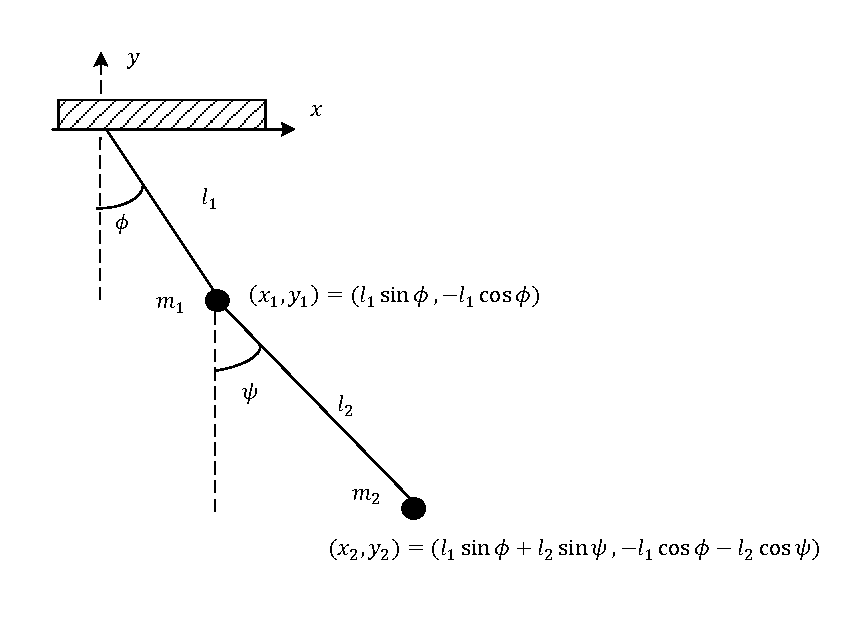
\includegraphics [width=10cm, height=8cm] {MyDoublePendulum}}
\caption{Pendulu bikoitz arrunta.}
\label{fig:dp}
\end{figure} 

\paragraph*{Hamiltondar funtzioa} $H(q,p)$  honakoa da,

\begin{multline}
 \label{eq:2}
-\frac{ {l_1}^2 \ (m_1+m_2) \ {p_{\theta}}^2 +{l_2}^2 \ m_2 \ (p_{\theta} -p_{\phi})^2 + 2 \ l_1 \ l_2 \ m_2 \ p_{\theta} \ (p_{\theta} -p_{\phi}) \  \cos(\theta )} {{l_1}^2  \ {l_2}^2 \ m_2 \  (-2 \ m_1 - m_2 + m_2 \ \cos(2 \theta ))} \\
-g  \ \cos (\phi) \  (l_1 \ (m_1+m_2)+l_2 \ m_2 \ \cos(\theta))+g \ l_2 \ m_2 \ \sin(\theta) \sin(\phi),
\end{multline}

\paragraph*{Sistemaren parametroak.} 
Gure esperimentuetarako honako parametroak kontsideratuko ditugu,
\begin{equation*}
 \label{eq:17}
g=9.8 \ {m}/{s^2}\ ,\ \ l_1=1.0 \ m \ , \ l_2=1.0 \ m\ , \ m_1=1.0 \ kg\ , \ m_2=1.0 \ kg.
\end{equation*} 

\paragraph*{Hasierako balioak.}
Bi hasierako balio ezberdin kontsideratu ditugu \cite{Dumitru}: lehenak, izaera ez-kaotikoa du eta bigarrenak, izaera kaotikoa duen mugimendua agertzen du.
\begin{enumerate}
   \item Hasierako balio ez-kaotikoak (NCDP): 
   \ $q(0)=(1.1, \ -1.1)$  eta $p(0)=( 2.7746,\ 2.7746)$. $T_{end}=2^{12}$ segundoko integrazioa egin dugu.
   
   \item Hasierako balio kaotikoak (CDP):      
    $q(0)=(0, \ 0)$ eta  $p(0)=(3.873,\ 3.873)$. $T_{end}=2^{8}$ segundoko integrazioa egin dugu.
\end{enumerate}

Urrats luzera, $h=2^{-7}$ aukeratu dugu, trunkatze errorea biribiltze errorea baino txikiagoa izan dadin.

\subsection{Pendulu bikoitz zurruna.}
\label{ss:322}

Pendulu bikoitz arruntari, malguki bat gehitutako sistema da (ikus \ref{fig:dp_zurruna}~irudia) :  $m_1$ eta $m_2$ masadun bi penduluk eta hauen artean $k$ parametroaren araberako malgutasuna duen malgukiak osatzen duten sistema mekanikoa. $k=0$ balioarentzat, problema ez da zurruna (hau da, pendulu bikoitz arrunta) eta problemaren zurruntasuna, $k$ balioarekin batera handitzen da. 

\begin{figure} [h]
\centerline{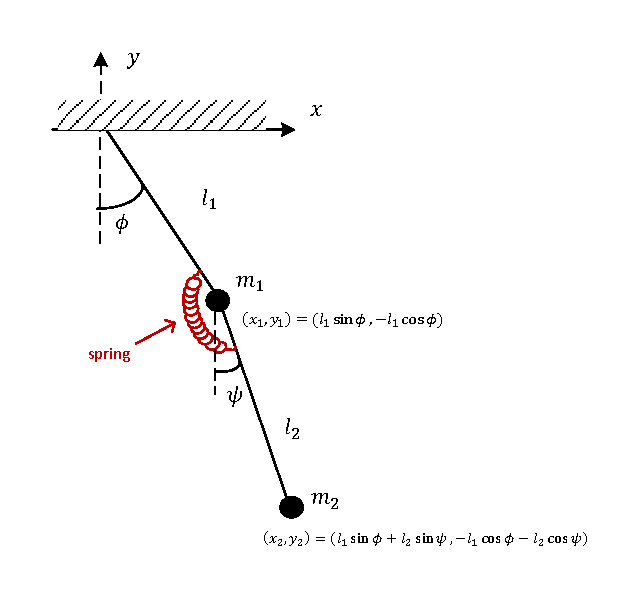
\includegraphics [width=10cm, height=8cm] {MyDoublePendulumSTIFF}}
\caption{Pendulu bikoitza (zurruna).}
\label{fig:dp_zurruna}
\end{figure} 

Sistemaren egoera aldagaiak, bi angelu $q=(\phi,\theta)$ eta dagozkion momentuak $p=(p_{\phi},p_{\theta})$ dira.  $\phi$ lehen penduluak ardatz bertikalarekiko duen angelua da eta bigarren penduluaren angelua, era honetan definituko dugu  $\psi=\phi+\theta$.

\paragraph*{Hamiltondar funtzioa.} 
Formulazio Lagrangiarrean ($L=T-V$), energia potentzialari $1/2 \ k \ \theta^2$ gaia gehituz, dagokion $H(q,p)$ funtzio Hamiltondarra lortuko dugu,
\begin{multline}
\label{eq:Hpb2}
-\frac{ {l_1}^2 \ (m_1+m_2) \ {p_{\theta}}^2 +{l_2}^2 \ m_2 \ (p_{\theta} -p_{\phi})^2 + 2 \ l_1 \ l_2 \ m_2 \ p_{\theta} \ (p_{\theta} -p_{\phi}) \  \cos(\theta )} {{l_1}^2  \ {l_2}^2 \ m_2 \  (-2 \ m_1 - m_2 + m_2 \ \cos(2 \theta ))} \\
-g  \ \cos (\phi) \  (l_1 \ (m_1+m_2)+l_2 \ m_2 \ \cos(\theta))+g \ l_2 \ m_2 \ \sin(\theta) \sin(\phi)+\frac{k}{2} \ \theta^2 ,
\end{multline}

\paragraph*{Sistemaren parametroak.} 
Honako parametroak kontsideratu ditugu,
\begin{equation*} \label{eq:17}
g=9.8 \ {m}/{s^2}\ ,\ \ l_1=1.0 \ m \ , \ l_2=1.0 \ m\ , \ m_1=1.0 \ kg\ , \ m_2=1.0 \ kg,
\end{equation*} 
eta $k$ malgutasun parametroaren balio batzuk finkatu ditugu, zurruntasun maila ezberdineko pendulu bikoitzaren dinamikak aztertzeko 
\begin{equation*}
k=2^{2i}, \ \ i=0,\dots,11.
\end{equation*}  

\paragraph*{Hasierako balioak.}
Hasierako balioak, era honetan aukeratu ditugu:
\begin{enumerate}
\item  $k=0$ problemarako, \cite{Dumitru} artikulutik izaera ez-kaotikoa duen hasierako balioak hartu ditugu: $q(0)=(1.1, -1.1)$ and $p(0)=(2.7746,2.7746)$.

\item  $k\neq 0$ problemetarako hasierako balioak,
\begin{equation*}
q(0)=\left(1.1, \frac{-1.1}{\sqrt{1+100k}}\right), \ \ 
p(0)=(2.7746,2.7746),
\end{equation*}
aukeratu ditugu, non sistemaren energia $k \rightarrow \infty$ doanean bornatua dagoen.

\end{enumerate}

$k=0$ problema ez-zurrunerako, $h=2^{-7}$ urrats luzera, trunkatze errorea biribiltze errorea baino txikiagoa izan dadin finkatu dugu eta gainontzeko integrazio guztietarako urrats luzera berdina erabili dugu. $k>0$ zurruntasun balio batetik aurrera, trunkatze errorea birbiltze errorea baino garrantzitsuago da. $T_{end}=2^{12}$  segundoko integrazioa egin dugu. 

\section{N-Gorputzen problema.}
\label{s:33}

Problemaren formulazioa eman aurretik, K.Tanikawa-k eta T.Ito-k \cite{Ito2007} 3-gorputzen problemari buruzko deskribapena aipatuko nahi genuke,

\begin{displayquote}
Never be attracted to the three-body problem. It is too dangerous. The three-body problem has long been an attractive but dangerous subject for students. This is because it has quite a simple setting and it appears relatively easy. However, it has been investigated for so many years that it is very difficult to obtain anything new.
\end{displayquote}

Newtonen lege grabitazionalen araberako N-gorputzen problemaren ekuazio diferentzialak era honetan definitzen dira,
\begin{equation}
m_i\ddot{q_i}= G \sum_{j=0,j \neq i}^{N} \frac{m_im_j}{\|q_j-q_i\|^3} (q_j-q_i) , \ \  i=0,1,\dots, N,
\end{equation}
non $(N+1)$ gorputz kopurua den, eta $q_i\in \mathbb{R}^3$, $m_i \in \mathbb{R}, \ \ i=0,\dots,N$ gorputz bakoitzaren kokapena eta masa den. 

\paragraph*{Hamiltondar sistema.}
Momentuen definizio hau ordezkatuz  $p_i=m_i*\dot{q}_i$, N-gorputzeko problemaren formulazio Hamiltondarra  lortzen da,  

\begin{equation}
H(q,p)=\frac{1}{2}\ \sum^N_{i=0}{\ \frac{{\|p_i\|}^2}{m_i}}-G\ \sum^N_{0\le i<j\le N}{\frac{m_im_j}{\|q_i-q_j\|}}. 
\end{equation}

\paragraph*{Ekuazio diferentzialak.} Abiaduraren eta kokapenaren araberako ekuazioak hauek dira,
\begin{align}
\label{eq:nbody}
\begin{split}
\dot{q}_i &=v_i, \ \  i=0,1,\dots, N,\\
\dot{v}_i &= \sum_{j=0,j \neq i}^{N} \frac{Gm_j}{\|q_j-q_i\|^3} (q_j-q_i) , \ \  i=0,1,\dots, N
\end{split}
\end{align}


\paragraph*{Problemaren integralak.}
Integrazioan zehar konstante mantentzen diren kantitateei problemaren integralak edo inbarianteak deitzen zaie. N-gorputzen problemak $10$ integral ditu \cite{Klioner2016}:
\begin{enumerate}


\item Masa zentroaren sei integralak.

Era honetan definitzen dugun $P$, konstantea dela modu errazean froga daiteke, 
\begin{equation*}
P=\sum_{i=0}^{N} m_i \dot{q}_i=\sum_{i=0}^{N} p_i. 
\end{equation*}
Eta ondorioz,
\begin{equation*}
O=\sum_{i=0}^{N} m_i {q}_i=Pt+B. 
\end{equation*}

$P,B \in \mathbb{R}^3$ bektoreen osagaiei, masa zentroaren sei integralak esaten zaie. Masa zentroaren kokapena ($Q$) eta abiadura ($V$)  era honetan definitzen dira, 
\begin{equation*}
Q=\frac{\left(\sum\limits_{i=0}^{N} m_i \ q_i\right)}{M}, \ V=\frac{\left(\sum\limits_{i=0}^{N} m_i \ \dot{q}_i\right)}{M}
\end{equation*}
non $M=\sum\limits_{i=0}^{N}Gm_i$ den.


\item Momentu angeluarra.

Momentu angeluarra $L\in \mathbb{R}^3$, problemaren beste hiru integralak dira, 
\begin{equation*}
L=\sum_{i=0}^{N} p_i \times q_i=\sum_{i=0}^{N} q_i \times m_i \dot{q}_i.
\end{equation*}

\item Energia.

Hamitondar sistema osoaren energia da eta problemaren beste integrala da,
\begin{equation*}
E=H(q,p).
\end{equation*}

\end{enumerate}

Problemaren $10$ integral hauek, sistemaren ordena gutxitzeko edo zenbakizko integrazioaren doitasuna neurtzeko erabil daitezke. Guk koordenatu barizentrikoak (koordenatu sistemaren jatorria masa zentroaren kokapena) erabiliko ditugu eta koordenatu hauetan, $P=0$ eta $B=0$ dira. Beraz, integratzeko erabiliko ditugun hasierako balioak ($\hat{q}_i,\hat{v}_i$) modu honetan finkatuko ditugu,
\begin{align*}
&\hat{q}_i=q_i-Q, \\
&\hat{v}_i=v_i-V, \ \ i=0,\dots,N,
\end{align*}
eta era honetan, masa zentroaren kokapen eta abiadurak,
\begin{equation*}
\hat{Q}=\frac{\left(\sum\limits_{i=0}^{N} m_i \ \hat{q}_i\right)}{M}=0, \ \hat{V}=\frac{\left(\sum\limits_{i=0}^{N} m_i \ \hat{v}_i\right)}{M}=0
\end{equation*}
izan daitezen,

Momentu angeluarra eta energia, zenbakizko integrazioaren doitasuna neurtzeko erabili ohi dira. Energia zenbakizko integrazioen biribiltze errorea neurtzeko integral egokiena da.

\section{Eguzki-sistema.}
\label{ss:34}

\subsection{Sarrera.}

Eguzki-sistemaren planeten orbiten mugimenduaren eredu matematikoa, sistema Hamiltondar bati dagokion ekuazio diferentzial arrunten bidez formulatzen da. $N$ planeta badaude, $6N$ ekuazio diferentzialeko sistema izango da.

Eguzki sistemaren eredu sinplea integratuko dugu. Eguzki-sistemaren gorputzak masa puntualak kontsideratuko ditugu eta gure ekuazio diferentzialak definitzeko, soilik gorputz hauen arteko erakarpen grabitazionalak hartu ditugu kontutan.

Eguzki-sistemaren gorputz nagusien (eguzkia eta planetak) integrazioetara mugatuko gara. Ereduen gorputz kopurua txikia izango da, kanpo-planeten probleman $N=6$ eta $9$-planeten probleman $N=10$ izango da.

Eguzkiak, planetak baino $1.000$ aldiz masa handiago du eta hauxe da, eguzki-sistemaren ezaugarri garrantzitsuenetakoa: eguzkiaren grabitazio indar nagusiak eta planeten arteko perturbazio txikiek sortzen duten sistema dinamikoa da. Planeten eta beren sateliteen mugimenduan kolisiotik gertuko egoerarik edo eszentrikotasun handiko orbitarik ez dago. Beraz, ikuspuntu honetatik sistema dinamiko sinplea dela, esan daiteke. Eguzki-sistema egonkorra kontsideratzen da, hau da, epe luze batean planeten arteko talkarik edo planeten kanporatzerik gertatzea, ez da espero  \cite{Laskar1999,Hayes2007}.

%Egonkortasunaren azterketa zehatzago batean, sistema erregularrak eta kaotikoak bereiz ditzakegu. Sistema erregularretan, hasierako balioen perturbazio txikien eragina, denboran zehar poliki hasiko da  eta beraz, epe luzeko integrazio zehatzak posible dira. Sistema kaotikoetan aldiz, eboluzioa hasierako balioekiko oso sentikorra da eta gertuko soluzioen diferentzia esponentzialki hasiko da. Hasierako uneko diferentzia $d(0)=d_0$ bada, orduan distantzia,
%\begin{equation*}
%d(t)\approx d(0)e^{t \lambda}
%\end{equation*}  
%espresioaren arabera hasiko da, non $\lambda$ \emph{Lyapunov esponentziala} esaten zaion. Eguzki-sistema kaotikoa kontsideratzen da eta Laskar-ek \cite{Laskar1999} \emph{Lyapunov denbora} $\lambda^{-1}\approx 5$ milioi urtetan finkatzen du eta honako espresioa, kalkulatzeko  proposatzen du,
%\begin{equation*}
%d(t)\approx d(0)10^{t / 10}.
%\end{equation*}     
%Espresio honen arabera,  $10^{-10}$ tamainako hasierako erroreak baditugu , orduan $d(10)\approx 10^{-9}$ eta $d(100)\approx 1$ dira. Ondorioz, eguzki sistemaren $10-20$ milioi urteko integrazioetarako, doitasun handiko soluzioak lortuko ditugu baina $100$ milioi urteko integrazioen soluzioak ez dira esanguratsuak izango.   

Eguzki-sistemaren jatorria, orain $5  \times 10^9$ urtetan finkatzen da eta beraz, eguzki-sistemaren eboluzioa integratzeko, urrats kopuru oso handia beharrezkoa da. Eguzki-sistemaren eredu osoaren (9-planeten problema) integrazioetako ohiko urratsa  $h=0.0025$ urtekoa bada (orbita txikieneko periodoaren $ \%1$), eman beharreko urrats kopurua $2 \times 10^{12}$ izango da. Era berean, eguzki-sistemaren eredu sinpleagoaren (kanpo-planeten problema) integrazioetako urrats tamaina handiago bada ere, urrats kopurua $5 \times 10^{10}$ ingurukoa da.   

Eguzki-sistemaren problemaren eskalak, anitzak dira. (\ref{fig:lbes}) irudian, planeta nagusien tamainak irudikatu ditugu eta (\ref{tab:eguz-sist}) taulan, eguzki-sistemaren planeten ezaugarri nagusienak eman ditugu. Aniztasunaren adierazgarri, ilargiaren, lurraren eta Neptunoren orbitak konpara ditzakegu: ilargiak $27.32$ eguneko periodoa duen orbita dauka, lurrak urtebetekoa eta Neptunok $163$ urtekoa.

\begin{figure} [h!]
\centerline{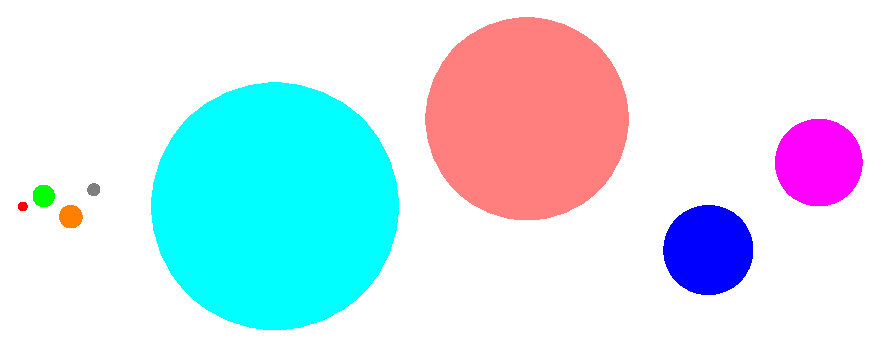
\includegraphics [width=8cm, height=3cm] {PanetenMasak}}
\caption{\small  Irudian, planeten arteko tamainen proportzioak irudikatu ditugu. Ezkerretik eskuinera: Merkurio, Artizarra, Lurra, Marte, Jupiter, Saturno, Urano eta Neptuno}
\label{fig:dp_zurruna}
\end{figure} 


\begin{table} [h!]
\caption{Eguzki-sistemaren planeta nagusien masak, eguzkiarekiko distantziak, orbitaren periodoa eta eszentrikotasuna.}
\label{tab:eguz-sist}       % Give a unique label
\begin{tabular}{l l l l l} 
\hline
 Planeta   &  Masak                 & Distantzia   & Periodoa    & Eszentrikotasuna\\   
           &  kg                    & AU           &   urteak    &               \\ \hline
 Eguzkia   &  $1.99 \times 10^{30}$ &              &             &               \\         
 Merkurio  &  $3.30 \times 10^{23}$ & $0.39$       &  $0.24$     &  $0.205$      \\
 Artizarra &  $4.87 \times 10^{24}$ & $0.72$       &  $0.007$    &  $0.007$      \\
 Lurra     &  $5.97 \times 10^{24}$ & $1.00$       &  $1.007$    &  $0.017$      \\
 Marte     &  $6.42 \times 10^{23}$ & $1.52$       &  $1.88$     &  $0.094$      \\ \hline
 Jupiter   &  $1.90 \times 10^{27}$ & $5.20$       &  $11.86$    &  $0.049$      \\
 Saturno   &  $5.68 \times 10^{26}$ & $9.54$       &  $29.42$    &  $0.057$      \\
 Urano     &  $8.68 \times 10^{25}$ & $19.19$      &  $83.75$    &  $0.046$      \\
 Neptuno   &  $1.02 \times 10^{26}$ & $30.06$      &  $163.72$   &  $0.011$      \\
 Pluton    &  $1.31 \times 10^{22}$ & $39.53$      &  $248.02$   &  $0.244$      \\
\hline
\end{tabular}
\end{table}

Hiru dira erabiltzen diren koordenatu sistema nagusienak:
\begin{enumerate}
\item Koordenatu cartesiarrak.
\item Koordenatu heliozentrikoak.
\item Koordenatu jacobiarrak.
\end{enumerate}

Ohikoa da ekuazio diferentzialak koordenatu heliozentrikoen (eguzkiaren zentroarekiko) arabera definitzea. 
Ekuazioen garapen osoa eranskinean eman dugu.

\subsection{Problemak.}
\label{ss:342}

Eguzki-sistemaren simulaziorako test problemak deskribatuko ditugu. Kanpo-planeten problematik abiatuta, gero eta problema konplexuagoak azalduko ditugu. PW, Sharp-ek \cite{Sharp2001} eguzki-sistemaren problemen bilduma interesgarria egin zuen, eta bertan problema hauek guztiak  problema ez-zurrunak kontsideratzen dituela nabarmentzekoa da.


\subsubsection*{Kanpo-planeten problema.}


Kanpo-planeten problemaren ereduan, eguzkia, lau planeta nagusiak (Jupiter, Saturno, Urano, Neptuno) eta Pluton kontsideratuko ditugu. Eguzki-sistemaren kanpo-planeten  mugimenduaren azterketa interesgarria da. Lehenik, planeta nagusi hauen eboluzioa eguzki-sistema osoaren zati garrantzitsuena da eta barne-planeten mugimendua kontutan hartzeak ala ez, kanpo-planeten zenbakizko integrazioarengan oso eragin txikia du. Bigarrenik, urrats luzera handia erabili daiteke eta beraz, epe luzeko integrazioak errazten dira (konputazio denbora gutxiago behar delako). Hirugarrenik, Pluton orbitaren berezitasunak ikertzea,  $1960-1980$ urteetan interes handikoa izan zen.        


Hasierako balioak \cite{Hairer2006} liburutik hartu ditugu. Planetei dagokien masak \ref{tab:ossm0} taulan eta kokapenak/abiadurak \ref{tab:oss0} taulan laburtu ditugu. planeten masak eguzkiarekiko erlatiboak dira, hau da, eguzkiaren masa $1$ da eta grabitazio konstantea $G=2.95912208286 \ 10^{-4}$. Barne-planeten masak eguzkiaren masari gehitu zaio eta horregatik, eguzkiaren masak, $m_0=1.00000597682$ balioa hartzen du.

\begin{table}[h]
\caption{Kanpo-planeten masak.}
\label{tab:ossm0}       % Give a unique label
\centering
\begin{tabular}{ l r }
\hline 
  Gorputza         &  Masa        
\\\hline
  Eguzkia          &  $1.000005976823$ \\
  Jupiter          &  $0.000954786104043$ \\
  Saturno          &  $0.000285583733151$ \\
  Urano            &  $0.0000437273164546$ \\
  Neptuno          &  $0.0000517759138449$ \\
  Pluton           &  ${1}/{(1.3 \ 10^8)}$ \\
\hline  
\end{tabular}
\end{table}

\begin{table}[h]
\caption[Kanpoko planeten problema.]{Kanpo-planeten problemaren hasierako balioak, kokapenak ($x,y,z$) eta abiadurak ($v_x,v_y,v_z$).}
\label{tab:oss0}       % Give a unique label
\centering
\resizebox{\textwidth}{!}{%
\begin{tabular}{ l l r r r }
\hline 
  Gorputza       &  Balioa \\
  \hline
  Eguzkia        &  $x,y,z$         & $0.$ & $0$ &	$0.$    \\
                 &  $v_x,v_y,v_z$   & $0.$ & $0.$ & $0.$    \\
  Jupiter        &  $x,y,z$         & $-3.5023653$ &  $-3.8169847$ & $-1.5507963$ \\
                 &  $v_x,v_y,v_z$   & $0.00565429$ &  $-0.00412490$ & $-0.00190589$ \\                    
  Saturno        &  $x,y,z$         &  $9.0755314$	& $-3.0458353$ & $-1.6483708$	    \\
                 &  $v_x,v_y,v_z$   &  $0.00168318$ & $0.00483525$ & $0.00192462$     \\
  Urano          &  $x,y,z$         &  $8.3101420$ & $-16.2901086$ & $-7.2521278$  \\
                 &  $v_x,v_y,v_z$   &  $0.00354178$ & $0.00137102$ & $0.00055029$ \\
  Neptuno        &  $x,y,z$         &  $11.4707666$ &	$-25.7294829$	& $-10.8169456$    \\
                 &  $v_x,v_y,v_z$   &  $0.00288930$  &	$0.00114527$ & $0.00039677$     \\
  Pluton         &  $x,y,z$         &  $-15.5387357$ &  $-25.2225594$ & $-3.1902382$ \\
                 &  $v_x,v_y,v_z$   &  $0.00276725$ &	$-0.00170702$ & $-0.00136504$ \\
\hline       
\end{tabular}}
\end{table}


\subsubsection*{9-planeten problema.}


Eguzki-sistemaren 9-planeten zenbakizko integrazioak, kanpo-planeten problemak baino konplexutasun handiago du. Planeten eta eguzkiaren arteko interakzio kopurua $45$ (kanpo-planeten probleman $15$) da. Planeten orbiten periodoen arteko aldea askoz handiago da. Merkurioren orbitaren eszentrikotasuna $e=0.206$ (Jupiterren orbitaren eszentrikotasuna $e=0.048$) da. 

Eredu honetan, lur-ilargi sistema (\emph{EMB}) masa puntual bakarra kontsideratzen da. Lur-ilargi sistemaren masa, bi gorputzen masen arteko batura da eta kokapena, lur-ilargi sistemaren barizentroan finkatzen da.
  
Hasierako balioak \emph{DE-430} ($2.014$) \cite{Folkner2014} azken efemeride artikulutik hartu ditugu. Eguzki eta planeten hasierako kokapenak (AU) eta abiadurak (AU/egun), (\ref{tab:9bodyhas}) taulan laburtu ditugu. Era berean, planeta bakoitzari dagokion $Gm$ balioa (\ref{tab:9bodymas}) taulan laburtu dugu. 

\begin{table}[h]
\caption{Planeten $GM$ balioak.}
\label{tab:9bodymas}       % Give a unique label
\centering
\begin{tabular}{l c }
\hline 
  Gorputza         &  GM ($au^3/day^3$)          \\
  \hline
  Eguzkia          &  $0.295912208285591100e-03$ \\
  Merkurio         &  $0.491248045036476000e-10$ \\
  Artizarra        &  $0.724345233264412000e-09$ \\
  Lurra            &  $0.888769244512563400e-09$ \\
  Marte            &  $0.954954869555077000e-10$ \\
  Jupiter          &  $0.282534584083387000e-06$ \\
  Saturno          &  $0.845970607324503000e-07$ \\
  Urano            &  $0.129202482578296000e-07$ \\
  Neptuno          &  $0152435734788511000e-07$ \\
  Pluton           &  $0.217844105197418000e-11$ \\
  Ilargia          &  $0.109318945074237400e-10$ \\
\hline
\end{tabular}
\end{table}

\begin{table}[h]
\caption[9-planeten problemaren hasierako balioak]{Eguzki eta 9 planeten hasierako balioak, kokapenak ($x,y,z$) (AU) eta abiadurak ($v_x,v_y,v_z$) (AU/egun). Julian data (TDB) $2440400.5$ ($1969$. ekainaren $28$) eta ICRFR2 (International Celestial Reference Frame) koordenatu sisteman emanak dira.}
\label{tab:9bodyhas}       % Give a unique label
\centering
\resizebox{\textwidth}{!}{%
\begin{tabular}{ l l r r r }
\hline 
  Gorputza       &  Balioa \\
  \hline
  Eguzkia        &  $x,y,z$         & $0.00450250878464055477$ & $0.00076707642709100705$ &	$0.00026605791776697764$    \\
                 &  $v_x,v_y,v_z$   & $-0.00000035174953607552$ & $0.00000517762640983341$ & $0.00000222910217891203$    \\
  Merkurio       &  $x,y,z$         &  $0.36176271656028195477$ & $-0.09078197215676599295$ &	$-0.08571497256275117236$ \\
                 &  $v_x,v_y,v_z$   &  $0.00336749397200575848$ & $0.02489452055768343341$ &	$0.01294630040970409203$ \\
  Artizarra      &  $x,y,z$         &  $0.61275194083507215477$ & $-0.34836536903362219295$	& $-0.19527828667594382236$ \\
                 &  $v_x,v_y,v_z$   &  $0.01095206842352823448$ & $0.01561768426786768341$ &	$0.00633110570297786403$\\
  EMB            &  $x,y,z$         &  $0.12051741410138465477$ & $-0.92583847476914859295$ &	$-0.40154022645315222236$\\
                 &  $v_x,v_y,v_z$   &  $0.01681126830978379448$ & $0.00174830923073434441$ &	$0.00075820289738312913$\\
  Marte          &  $x,y,z$         & $-0.11018607714879824523$ & $-1.32759945030298299295$ &	$-0.60588914048429142236$ \\
                 &  $v_x,v_y,v_z$   &  $0.01448165305704756448$ & $0.00024246307683646861$ & $-0.00028152072792433877$   \\
  Jupiter        &  $x,y,z$         &  $-5.37970676855393644523$ & $-0.83048132656339789295$ & $-0.22482887442656542236$ \\
                 &  $v_x,v_y,v_z$   & $0.00109201259423733748$ & $-0.00651811661280738459$ &	$-0.00282078276229867897$\\                  
  Saturno        &  $x,y,z$         &  $7.89439068290953155477$ & $4.59647805517127300705$ &	$1.55869584283189997764$	    \\
                 &  $v_x,v_y,v_z$   &  $-0.00321755651650091552$ & $0.00433581034174662541$ & $0.00192864631686015503$     \\
  Urano          &  $x,y,z$         &  $-18.26540225387235944523$ &	$-1.16195541867586999295$ &	 $-0.25010605772133802236$\\
                 &  $v_x,v_y,v_z$   &  $0.00022119039101561468$ & $-0.00376247500810884459$ &	$-0.00165101502742994997$ \\
  Neptuno        &  $x,y,z$         &  $-16.05503578023336944523$ &	$-23.94219155985470899295$ &	 $-9.40015796880239402236$    \\
                 &  $v_x,v_y,v_z$   & $0.00264276984798005548$ & $-0.00149831255054097759$ &	$-0.00067904196080291327$     \\
  Pluton         &  $x,y,z$         &  $-30.48331376718383944523$ & $-0.87240555684104999295$ &	 $8.91157617249954997764$ \\
                 &  $v_x,v_y,v_z$   &  $0.00032220737349778078$ & $-0.00314357639364532859$ &	$-0.00107794975959731297$\\
\hline       
\end{tabular}}
\end{table}
                 


\subsubsection*{Laskar-en eredua.}

Eguzki-sistemaren mugimenduaren azterketa zehatza egiteko, planeten eta ilargiaren orbiten mugimenduaren ekuazioak nahiz lur eta ilargiaren errotazio mugimenduaren ekuazioak integratu behar dira. 

Laskar-ek, $2.011.$ urteko epe luzeko zenbakizko integraziorako \cite{Laskar2011} eguzki-sistemaren eredua deskribatuko dugu. Hasierako integrazioetan, eguzkia, 8 planetak, Pluton eta ilargia bakarrik kontsideratu zituen. Eguzkiaren erlatibitate efektua (Saha eta Tremain-ek \cite{Saha1994} finkatutako teknikaren arabera) eta eredu errealistaren indar ez grabitazional garrantzitsuenak aplikatu zituen. Azken integrazioetan, Zeres, Palas, Vesta, Iris eta Bamberga asteroideak gehitu zituen.  
 

\begin{table} [h!]
\caption{}
\label{tab:laskp}       % Give a unique label
\begin{tabular}{l r r r r } 
\hline
 Planeta   &  Distantzia   & Periodoa    & GM             & Ezentrizitatea \\   
           &   AU          &   urte      & ($au^3/egun^3$) & \\ \hline
 Eguzkia    &               &             & $0.2959e-03$   & \\          
 Merkurio   &   $0.39$      &  $0.24$     & $0.4912e-10$   & $0.205$ \\
 Artizarra  &   $0.72$      &  $0.007$    & $0.7243e-09$   & $0.007$\\
 Lurra      &   $1.00$      &  $1.007$    & $0.8887e-09$   & $0.017$\\
 Ilargia    &               &             & $0.1093e-10$   & $0.055$\\ 
 Marte      &   $1.52$      &  $1.88$     & $0.9549e-10$   & $0.094$\\ \hline
 Jupiter    &   $5.20$      &  $11.86$    & $0.2825e-06$   & $0.049$\\
 Saturno    &   $9.54$      &  $29.42$    & $0.8459e-07$   & $0.057$\\ 
 Urano      &   $19.19$     &  $83.75$    & $0.1292e-07$   & $0.046$\\
 Neptuno    &   $30.06$     &  $163.72$   & $0.1524e-07$   & $0.011$ \\ \hline
 Zeres      &   $2.77$      &  $4.6$      & $0.1400e-12$   & $0.07$ \\
 Palas      &   $2.77$      &  $4.61$     & $0.3104e-13$   & $0.23$ \\
 Vesta      &   $2.36$      &  $3.63$     & $0.3854e-13$   & $0.08$\\
 Iris       &   $2.38$      &  $3.68$     & $0.2136e-14$   & $0.21$ \\
 Bamberga   &   $2.68$      &  $4.39$     & $0.1388e-14$   & $0.34$ \\ \hline
 Pluton     &   $39.53$     &  $248.02$   & $0.2178e-11$   & $0.244$ \\
\hline
\end{tabular}
\end{table}

Ilargia gorputz independente gisa kontsideratu zuen. Ilargiaren lurrarekiko distantzia ($380.000$ km) , beste gorputzekiko distantziekin alderatzen badugu (eguzkiarekiko $150.000.000$ km eta Artizarrarekiko $45.000.000$ km) oso txikia da. Hori dela eta, ilargiaren kokapena, eguzki-sistemaren barizentroarekiko kontsideratu ordez, lurrarekiko kontsideratuz doitasun handiagoa lortuko da. Lurraren eguzkiarekiko kokapena ($q_e$) eta ilargiaren eguzkiarekiko kokapen ($q_m$), hurrenez-hurren, lur-ilargi sistemaren barizentroaren eguzkiarekiko kokapena ($q_B$) eta  ilargiaren lurrarekiko kokapena ($q_{em}$) aldagaiekin ordezkatzen dira,
\begin{align*}
& q_B =\frac{Gm_e \ q_e+Gm_m \ q_m}{Gm_e+Gm_m},\\
& q_{em} =q_m-q_e.
\end{align*}
Argitzea komeni da, ekuazio diferentzialaren eskubiko aldeko espresioa ebaluatzeko ($q_e,q_m$) aldagaiak erabiliko ditugula eta ($q_B,q_{em}$) aldagai berriak  integratzeko erabiliko ditugula.

\begin{algorithm}[H]
 \BlankLine
  $\mbox{Lurra, Ilargia}=\{q_B,q_{em}\}$\;
  \For{$i\leftarrow 1$ \KwTo $endstep$}
  {
   \BlankLine
     $\{q_e,q_m\} \leftarrow \{q_B,q_{em}\} $\;
     $\mbox{Ebaluatu} \ \dot{y}=f(y)$\;
     $ \{q_B,q_{em}\} \leftarrow \{q_e,q_m\} $\;
     $\mbox{Integrazioa}\ (q_B,q_{em})$\;
   \BlankLine
  }
 \caption{Ilargiaren kalkuluak.}
\end{algorithm}

\begin{table}[h]
\caption{Ilargiaren Lurrarekiko hasierako balioak.}
\label{tab:1}       % Give a unique label
\centering
\resizebox{\textwidth}{!}{%
\begin{tabular}{ c l c c c }
\hline 
  Gorputza       &  Balioa \\
\hline
  Ilargia        &  $x,y,z$         & $-0.00080817735147818490$ &	$-0.00199462998549701300$ &	$-0.00108726268307068900$    \\
                 &  $v_x,v_y,v_z$   & $0.00060108481561422370$ & $-0.00016744546915764980$ &	$-0.00008556214140094871$ \\
\hline
\end{tabular}}
\end{table}     
          

\section{Laburpena.}

Atal honetan, pendulu bikoitzaren problema eta eguzki-sistema grabitazionalaren eredu ezberdinen zehaztasunak eman ditugu. Batetik, pendulu bikoitzaren problemaren hasierako balioak \cite{Dumitru} artikulutik hartu ditugu. Bestetik, eguzki-sistema grabitazionalaren problemaren integraziorako hasierako balioak lan hauetatik hartu ditugu: kanpo-planeten problemarentzat \cite{Hairer2006} liburutik eta 9-planeten problemarentzat $2014.$ urteko efemerideen \cite{Folkner2014} artikulutik hartu ditugu. Eguzki-sistemaren problemaren integraziorako hasierako balioak jasotzen dituzten beste lan hauek ere aipatu nahi genituzke: P.W. Sharp-ek eguzki-sistemaren problemen bilduma \cite{Sharp2001} eta Laskar-en \cite{Laskar2009} artikuluaren informazio osagarria.